\documentclass[fleqn,8pt,t]{beamer}

\usepackage[english]{babel}
\usepackage[utf8]{inputenc}
\usepackage[T1]{fontenc}
%\usepackage{french} % Sommaire en début de document
%\usepackage[top=2cm, bottom=2cm, left=2cm, right=2cm]{geometry} % Marges

\usepackage{amsmath} % Maths
\usepackage{amsfonts} % Maths
\usepackage{amssymb} % Maths
\usepackage{stmaryrd} % Maths (crochets doubles)

%\usepackage{listings} % Mise en forme du code (pour Hoare) ## À REVOIR ###
%\usepackage{ifthen} % Structures If Then Else
\usepackage{theorem} % Styles supplémentaires pour théorèmes
\usepackage{url}
\usepackage{array}  % Tableaux évolués
\usepackage{multirow}  % Pour des colonnes sur plusieurs lignes

%\usepackage{enumerate} % Changer les puces des listes d'énumération
%\usepackage{setspace} % Changer les interlignes

%\usepackage{subfig} % Créer des sous-figures
%\usepackage{graphicx} % Importer des images

\usepackage{ulem}  % Pour l'attribut barré

\usepackage{comment}

% Police
\usepackage{lmodern}
%\usepackage{libertine}


%%%%%%%%%%%%%%%%%%%%%%%%%%%%%%%%%%%%%%
\usepackage{tikz}
\newdimen\pgfex
\newdimen\pgfem
\usetikzlibrary{arrows,shapes,shadows,scopes}
\usetikzlibrary{positioning}
\usetikzlibrary{matrix}
\usetikzlibrary{decorations.text}
\usetikzlibrary{decorations.pathmorphing}

\input{../macros}
\input{../macros-ph}
\input{../macros-abstr}

\def\Pint{\textsc{PINT}}
\def\PH{\mathcal{PH}}

\tikzstyle{sort}=[fill=lightgray, rounded corners, draw=black]
\tikzstyle{process}=[circle,draw,minimum size=15pt,font=\footnotesize,inner sep=1pt]
\tikzstyle{black process}=[process, draw=blue, fill=red,text=black,font=\bfseries]
\tikzstyle{highlighted process}=[current process, fill=gray]
\tikzstyle{process box}=[fill=none,draw=black,rounded corners]
\tikzstyle{current process}=[process,fill=blue]
\tikzstyle{tick label}=[font=\footnotesize]
\tikzstyle{tick}=[densely dotted]
\tikzstyle{hit}=[->,>=angle 45]
\tikzstyle{selfhit}=[min distance=30pt,curve to]
\tikzstyle{bounce}=[densely dotted,>=stealth',->]
\tikzstyle{hlhit}=[very thick]
\tikzstyle{ulhit}=[draw=lightgray,fill=lightgray]
\tikzstyle{pulhit}=[fill=lightgray]
\tikzstyle{bulhit}=[draw=lightgray]

\tikzstyle{hitless graph}=[every edge/.style={draw=red,-}]

\tikzstyle{aS}=[every edge/.style={draw,->}]
\tikzstyle{Asol}=[draw,circle,minimum size=5pt,inner sep=0]
\tikzstyle{Aproc}=[draw]
\tikzstyle{Aobj}=[]

\renewcommand{\TState}[2]{
  \foreach \proc in {#2} {
        \only<#1>{ \node[current process] (\proc) at (\proc.center) {}; }
  };
}

%\definecolor{darkred}{rgb}{0.5,0,0}
\definecolor{lightred}{rgb}{1,0.8,0.8}
\definecolor{lightgreen}{rgb}{0.7,1,0.7}
\definecolor{darkgreen}{rgb}{0,0.5,0}
\definecolor{darkblue}{rgb}{0,0,0.5}
\definecolor{darkyellow}{rgb}{0.5,0.5,0}
\definecolor{lightyellow}{rgb}{1,1,0.6}
\definecolor{darkcyan}{rgb}{0,0.6,0.6}
\definecolor{darkorange}{rgb}{0.8,0.2,0}

\definecolor{notsodarkgreen}{rgb}{0,0.7,0}

%\definecolor{coloract}{rgb}{0,1,0}
%\definecolor{colorinh}{rgb}{1,0,0}
\colorlet{coloract}{darkgreen}
\colorlet{colorinh}{red}
\colorlet{coloractgray}{lightgreen}
\colorlet{colorinhgray}{lightred}
\colorlet{colorinf}{darkgray}
\colorlet{coloractgray}{lightgreen}
\colorlet{colorinhgray}{lightred}

\colorlet{colorgray}{lightgray}


\tikzstyle{grn}=[every node/.style={circle,draw=black,outer sep=2pt,minimum
                size=15pt,text=black}, node distance=1.5cm]
\tikzstyle{inh}=[>=|,-|,draw=colorinh,thick, text=black,label]
\tikzstyle{act}=[->,>=triangle 60,draw=coloract,thick,color=coloract]
\tikzstyle{inhgray}=[>=|,-|,draw=colorinhgray,thick, text=black,label]
\tikzstyle{actgray}=[->,>=triangle 60,draw=coloractgray,thick,color=coloractgray]
\tikzstyle{inf}=[->,draw=colorinf,thick,color=colorinf]
%\tikzstyle{elabel}=[fill=none, above=-1pt, sloped,text=black, minimum size=10pt, outer sep=0, font=\scriptsize,draw=none]
\tikzstyle{elabel}=[fill=none,text=black, above=-2pt,%sloped,
minimum size=10pt, outer sep=0, font=\scriptsize, draw=none]
%\tikzstyle{elabel}=[]


\tikzstyle{plot}=[every path/.style={-}]
\tikzstyle{axe}=[gray,->,>=stealth']
\tikzstyle{ticks}=[font=\scriptsize,every node/.style={gray}]
\tikzstyle{mean}=[thick]
\tikzstyle{interval}=[line width=5pt,red,draw opacity=0.7]
\definecolor{lightred}{rgb}{1,0.3,0.3}

\tikzstyle{hl}=[yellow]
\tikzstyle{hl2}=[orange]

\tikzstyle{every matrix}=[ampersand replacement=\&]
\tikzstyle{shorthandoff}=[]
\tikzstyle{shorthandon}=[]
%%%%%%%%%%%%%%%%%%%%%%%%%%%%%%%%%%%%%%%%



% Commande À FAIRE
\usepackage{color} % Couleurs du texte
%\newcommand{\afaire}[1]{\textcolor{red}{[À FAIRE : #1]}}
\newcommand{\todo}[1]{\textcolor{red}{<[[#1]]>}}



\colorlet{couleurtheme}{gray}  % Couleur principale du thème
\colorlet{couleurcit}{gray}  % Couleur des citations
\colorlet{couleurex}{blue}  % Couleur des citations
\colorlet{couleurliens}{darkblue}  % Couleur des citations

\usetheme{Pittsburgh}   % Thème général
\usefonttheme{default}  % Thème de polices
\setbeamertemplate{navigation symbols}{}  % Pas de menu de navigation
%\setbeamertemplate{itemize item}[x]   % Puces des listes

\usecolortheme[named=couleurtheme]{structure}    % Couleur de la structure : titres et puces
%\setbeamercolor{normal text}{bg=black,fg=white}  % Couleur du texte
\setbeamercolor{item}{fg=couleurtheme}           % Couleur des puces
%\setbeamercolor{item projected}{fg=black}        % Couleur des recouvrements
%\setbeamercolor{alerted text}{fg=yellow}         % ?

\setbeamerfont{frametitle}{size=\Large}  % Police des titres


% Flèche grise
\newcommand{\f}{\textcolor{couleurtheme}{\textbf{$\rightarrow$\ }}}

% Environnement liste avec flèches
\newenvironment{fleches}{%
\begin{list}{}{%
\setlength{\labelwidth}{1em}% largeur de la boîte englobant le label
\setlength{\labelsep}{0pt}% espace entre paragraphe et l’étiquette
%\setlength{\itemsep}{1pt}
%\setlength{\leftmargin}{\labelwidth+\labelsep}% marge de gauche
\renewcommand{\makelabel}{\f}%
}}{\end{list}}

% Liste sans puce
\newenvironment{liste}{%
\begin{list}{}{%
\setlength{\labelwidth}{0em}% largeur de la boîte englobant le label
\setlength{\labelsep}{0pt}% espace entre paragraphe et l’étiquette
\setlength{\leftmargin}{0em}% marge de gauche
%\renewcommand{\makelabel}{\f}%
}}{\end{list}}

% Style des exemples
\newcommand{\ex}[1]{\textcolor{couleurex}{#1}}
\newcommand{\qex}[1]{\quad \ex{#1}}
\newcommand{\rex}[1]{\hfill \ex{#1}}
\newcommand{\redex}[1]{\textcolor{red}{#1}}

\newcommand{\lien}[1]{\textcolor{couleurliens}{\underline{\url{#1}}}}

\newcommand{\console}[1]{\textcolor{darkgray}{#1}}

% Style des citations
\newcommand{\tscite}[1]{\textcolor{couleurcit}{#1}}
\newcommand{\tcite}[1]{\textcolor{couleurcit}{[#1]}}

% Style de texte mis en valeur
\newcommand{\tval}[1]{\textbf{#1}}

% Un vrai symbole pour l'ensemble vide
\renewcommand{\emptyset}{\varnothing}

% Pour définir la conférence et son nom court
\newcommand{\conference}[2]{\def\theconference{#2}
\def\insertshortconference{\ifthenelse{\equal{#1}{-}}{#2}{\ifthenelse{\equal{#1}{}}{#2}{#1}}}}



\newcommand{\thedate}{2012/12/06}
\date{\thedate}
\conference{MOVEP'2012}{--- MOVEP'2012 ---\\10\textsuperscript{th} School for young researchers about\\Modelling and Verifying Parallel processes}
\title[Inferring BRNs from PH models]{Inferring Biological Regulatory Networks\\from Process Hitting models}
\author{Maxime FOLSCHETTE}




\setbeamertemplate{footline}{\color{gray}%
\scriptsize
\quad\strut%
\insertauthor%
\hfill%
\insertframenumber/\inserttotalframenumber%
\hfill%
\insertshortconference{} --- \thedate\quad\strut
}


\newcommand{\headersep}{$\circ$} % \bullet \triangleright

\setbeamertemplate{headline}{\color{gray}%
\vskip0.3em%
\quad\strut%
{\scriptsize\color{black}%
% Gris si une section existe
\ifthenelse{\equal{\thesection}{0}}{}{%
\ifthenelse{\equal{\lastsection}{x}}{}{%
\color{gray}%
}}%
\insertshorttitle
\ifthenelse{\equal{\thesection}{0}}{}{%
\ifthenelse{\equal{\lastsection}{x}}{}{%
~\headersep{} %
% Gris si une sous-section existe
\ifthenelse{\equal{\thesubsection}{0}}{\color{black}}{%
\ifthenelse{\equal{\lastsubsection}{x}}{\color{black}}{%
\color{gray}%
}}%
\insertsectionhead%
%
\ifthenelse{\equal{\thesubsection}{0}}{}{%
\ifthenelse{\equal{\lastsubsection}{x}}{}{%
~\headersep{} \color{black}\insertsubsectionhead%
%
}}}}}%
\vskip-5ex%
}



\def \scaleex {0.85}
\def \scaleinf {0.6}

\colorlet{colorb}{blue}
\colorlet{colora1}{yellow}
\colorlet{colora0}{green}
\colorlet{colora1font}{darkyellow}
\colorlet{colora0font}{darkgreen}

\colorlet{exanswer}{blue}
\colorlet{colorgray}{lightgray}

\definecolor{colortitle}{rgb}{0.54,0.8,0.9}


\begin{document}

\begin{frame}[plain,label=title]

% Cadre de titre
\begin{center}
\vspace{1cm}
\setbeamercolor{postit}{fg=black,bg=colortitle}
\begin{beamercolorbox}[sep=0.5em]{postit}
\centering
\Large
\textbf{%
{\normalsize\theconference{}}\\~\\%
\inserttitle
}
\end{beamercolorbox}

% Auteurs et instituts
\par
\medskip
\bigskip
\normalsize
Maxime FOLSCHETTE$^{1,2}$

\medskip
\footnotesize
MeForBio / IRCCyN / École Centrale de Nantes (Nantes, France)

\texttt{maxime.folschette@irccyn.ec-nantes.fr}

\url{http://www.irccyn.ec-nantes.fr/~folschet/}

\bigskip
Joint work with:
\\
\normalsize
Loïc PAULEVÉ, Katsumi INOUE, Morgan MAGNIN, Olivier ROUX
\end{center}

\end{frame}


% Exemples

%%% Exemple pour la définition du Process Hitting %%%
\def \exphdef {
\path[use as bounding box] (-0.5,-0.5) rectangle (6.5,4.5);

\TSort{(0,3)}{a}{2}{l}
\TSort{(0,0)}{b}{2}{l}
\TSort{(6,1)}{z}{3}{r}

\THit{a_1}{}{z_1}{.west}{z_2}
\THit{b_1}{}{z_0}{.west}{z_1}
\THit{a_0}{out=250,in=200,selfhit}{a_0}{.west}{a_1}

\path[bounce,bend left]
\TBounce{z_0}{}{z_1}{.south}
\TBounce{z_1}{}{z_2}{.south}
\TBounce{a_0}{}{a_1}{.south}
;
}



%%% Exemple pour la coopération %%%
\def \exphcoop {
\path[use as bounding box] (-0.5,-0.5) rectangle (6.5,4.5);

% Actions de màj grisées
\only<6->{
\THit{a_1}{ulhit,color=lightgray}{ab_0}{.west}{ab_2}
\THit{a_1}{ulhit,color=lightgray}{ab_1}{.west}{ab_3}
\path[bounce,bend left,pulhit] \TBounce{ab_0}{bulhit}{ab_2}{.south} \TBounce{ab_1}{bulhit}{ab_3}{.south} ;
}

\only<7->{
\THit{a_0}{ulhit}{ab_2}{.west}{ab_0}
\THit{a_0}{ulhit}{ab_3}{.west}{ab_1}
\path[bounce,bend right,pulhit] \TBounce{ab_2}{bulhit}{ab_0}{.north} \TBounce{ab_3}{bulhit}{ab_1}{.north} ;
}

\only<8->{
\THit{b_0}{ulhit}{ab_3}{.west}{ab_2}
\THit{b_0}{ulhit}{ab_1}{.west}{ab_0}
\THit{b_1}{ulhit}{ab_0}{.west}{ab_1}
\THit{b_1}{ulhit}{ab_2}{.west}{ab_3}
\path[bounce,bend right,pulhit] \TBounce{ab_1}{bulhit}{ab_0}{.north} \TBounce{ab_3}{bulhit}{ab_2}{.north} ;
\path[bounce,bend left,pulhit] \TBounce{ab_0}{bulhit}{ab_1}{.south} \TBounce{ab_2}{bulhit}{ab_3}{.south} ;
}

% Sortes
\TSort{(0,3)}{a}{2}{l}
\TSort{(0,0)}{b}{2}{l}
\TSort{(6,1)}{z}{3}{r}

% Deux actions disjointes en exemple
\only<2-3>{
\THit{a_1}{}{z_1}{.north west}{z_2}
\path[bounce,bend left]
\TBounce{z_1}{}{z_2}{.south} ;

\THit{b_0}{}{z_1}{.west}{z_2}
\path[bounce,bend left=55]
\TBounce{z_1}{}{z_2}{.south west} ;
}

% Processus d'exemple
\TState{3}{a_1,b_1,z_1}

% Sorte coopérative et arcs
\only<4->{
\TSetTick{ab}{0}{00}
\TSetTick{ab}{1}{01}
\TSetTick{ab}{2}{10}
\TSetTick{ab}{3}{11}
\TSort{(3,0.5)}{ab}{4}{l}
}

% Arcs de màj noirs de la sc
\only<5>{
\THit{a_1}{thick}{ab_0}{.west}{ab_2}
\THit{a_1}{thick}{ab_1}{.west}{ab_3}
\path[bounce,thick,bend left] \TBounce{ab_0}{thick}{ab_2}{.south} \TBounce{ab_1}{thick}{ab_3}{.south} ;
}

\only<6>{
\THit{a_0}{thick}{ab_2}{.west}{ab_0}
\THit{a_0}{thick}{ab_3}{.west}{ab_1}
\path[bounce,thick,bend right] \TBounce{ab_2}{thick}{ab_0}{.north} \TBounce{ab_3}{thick}{ab_1}{.north} ;
}

\only<7>{
\THit{b_0}{thick}{ab_3}{.west}{ab_2}
\THit{b_0}{thick}{ab_1}{.west}{ab_0}
\THit{b_1}{thick}{ab_0}{.west}{ab_1}
\THit{b_1}{thick}{ab_2}{.west}{ab_3}
\path[bounce,thick,bend right] \TBounce{ab_1}{thick}{ab_0}{.north} \TBounce{ab_3}{thick}{ab_2}{.north} ;
\path[bounce,thick,bend left] \TBounce{ab_0}{thick}{ab_1}{.south} \TBounce{ab_2}{thick}{ab_3}{.south} ;
}

% État d'exemple pour màj de la sc
\TState{8-9}{a_1,b_0}
\TState{10}{a_1,b_0,ab_0,ab_1,ab_2,ab_3}
\TState{11}{a_1,b_0,ab_2}
\only<9-11>{
\THit{a_1}{}{ab_0}{.west}{ab_2}
\THit{a_1}{}{ab_1}{.west}{ab_3}
\THit{b_0}{}{ab_3}{.west}{ab_2}
\THit{b_0}{}{ab_1}{.west}{ab_0}
\path[bounce,bend left] \TBounce{ab_0}{}{ab_2}{.south} \TBounce{ab_1}{}{ab_3}{.south} ;
\path[bounce,bend right] \TBounce{ab_1}{}{ab_0}{.north} \TBounce{ab_3}{}{ab_2}{.north} ;
}

% État d'exemple pour action de la sc
\TState{12}{a_1,b_0,z_1,ab_2}
\TState{13-14}{a_1,b_0,z_2,ab_2}

% Arc sortant de la sc
\only<12-14>{
\THit{ab_2}{thick}{z_1}{.west}{z_2}
\path[bounce,bend left,thick] \TBounce{z_1}{thick}{z_2}{.south} ;
}

% Arc sortant de la sc
%\only<15->{
%\THit{ab_2}{}{z_1}{.west}{z_2}
%\path[bounce,bend left] \TBounce{z_1}{}{z_2}{.south} ;
%}

}



%%% Exemple pour l'inférence %%%
\def \exphinf {
% Sortes
\TSort{(0,3)}{a}{2}{l}
\TSort{(0,0)}{b}{2}{l}
\TSort{(6,0)}{z}{3}{r}

% Sorte coopérative et arcs
\TSetTick{ab}{0}{00}
\TSetTick{ab}{1}{01}
\TSetTick{ab}{2}{10}
\TSetTick{ab}{3}{11}
\TSort{(3,0)}{ab}{4}{l}

% Actions de màj grisées
\THit{a_1}{ulhit}{ab_0}{.west}{ab_2}
\THit{a_1}{ulhit}{ab_1}{.west}{ab_3}
\path[bounce,bend left,pulhit] \TBounce{ab_0}{bulhit}{ab_2}{.south} \TBounce{ab_1}{bulhit}{ab_3}{.south};

\THit{a_0}{ulhit}{ab_2}{.west}{ab_0}
\THit{a_0}{ulhit}{ab_3}{.west}{ab_1}
\path[bounce,bend right,pulhit] \TBounce{ab_2}{bulhit}{ab_0}{.north} \TBounce{ab_3}{bulhit}{ab_1}{.north};

\THit{b_0}{ulhit}{ab_3}{.west}{ab_2}
\THit{b_0}{ulhit}{ab_1}{.west}{ab_0}
\THit{b_1}{ulhit}{ab_0}{.west}{ab_1}
\THit{b_1}{ulhit}{ab_2}{.west}{ab_3}
\path[bounce,bend right,pulhit] \TBounce{ab_1}{bulhit}{ab_0}{.north} \TBounce{ab_3}{bulhit}{ab_2}{.north};
\path[bounce,bend left,pulhit] \TBounce{ab_0}{bulhit}{ab_1}{.south} \TBounce{ab_2}{bulhit}{ab_3}{.south};

% Arcs sortant de la sc
\THit{ab_2}{ulhit}{z_1}{.north west}{z_2}
\THit{ab_2}{ulhit}{z_0}{.west}{z_1}
\path[bounce,bend left,pulhit] \TBounce{z_1}{bulhit}{z_2}{.south} \TBounce{z_0}{bulhit}{z_1}{.south};

\THit{ab_3}{ulhit}{z_2}{.west}{z_1}
\THit{ab_3}{ulhit}{z_0}{.west}{z_1}
\THit{ab_1}{ulhit}{z_2}{.west}{z_1}
\THit{ab_1}{ulhit}{z_0}{.west}{z_1}
\path[bounce,bend left,pulhit] \TBounce{z_2}{bulhit,bend right}{z_1}{.north};

\THit{ab_0}{ulhit}{z_2}{.west}{z_1}
\THit{ab_0}{ulhit}{z_1}{.south west}{z_0}
\path[bounce,bend right,pulhit] \TBounce{z_2}{bulhit}{z_1}{.north} \TBounce{z_1}{bulhit}{z_0}{.north};

}



%%% Exemple pour l'inférence (sans arcs grisés) %%%
\def \exphinfblack {
% Sortes
\TSort{(0,3)}{a}{2}{l}
\TSort{(0,0)}{b}{2}{l}
\TSort{(6,0)}{z}{3}{r}

% Sorte coopérative et arcs
\TSetTick{ab}{0}{00}
\TSetTick{ab}{1}{01}
\TSetTick{ab}{2}{10}
\TSetTick{ab}{3}{11}
\TSort{(3,0)}{ab}{4}{l}

% Actions de màj grisées
\THit{a_1}{}{ab_0}{.west}{ab_2}
\THit{a_1}{}{ab_1}{.west}{ab_3}
\path[bounce,bend left] \TBounce{ab_0}{}{ab_2}{.south} \TBounce{ab_1}{}{ab_3}{.south};

\THit{a_0}{}{ab_2}{.west}{ab_0}
\THit{a_0}{}{ab_3}{.west}{ab_1}
\path[bounce,bend right] \TBounce{ab_2}{}{ab_0}{.north} \TBounce{ab_3}{}{ab_1}{.north};

\THit{b_0}{}{ab_3}{.west}{ab_2}
\THit{b_0}{}{ab_1}{.west}{ab_0}
\THit{b_1}{}{ab_0}{.west}{ab_1}
\THit{b_1}{}{ab_2}{.west}{ab_3}
\path[bounce,bend right] \TBounce{ab_1}{}{ab_0}{.north} \TBounce{ab_3}{}{ab_2}{.north};
\path[bounce,bend left] \TBounce{ab_0}{}{ab_1}{.south} \TBounce{ab_2}{}{ab_3}{.south};

% Arcs sortant de la sc
\THit{ab_2}{}{z_1}{.north west}{z_2}
\THit{ab_2}{}{z_0}{.west}{z_1}
\path[bounce,bend left] \TBounce{z_1}{}{z_2}{.south} \TBounce{z_0}{}{z_1}{.south};

\THit{ab_3}{}{z_2}{.west}{z_1}
\THit{ab_3}{}{z_0}{.west}{z_1}
\THit{ab_1}{}{z_2}{.west}{z_1}
\THit{ab_1}{}{z_0}{.west}{z_1}
\path[bounce,bend left] \TBounce{z_2}{,bend right}{z_1}{.north};

\THit{ab_0}{}{z_2}{.west}{z_1}
\THit{ab_0}{}{z_1}{.south west}{z_0}
\path[bounce,bend right] \TBounce{z_2}{}{z_1}{.north} \TBounce{z_1}{}{z_0}{.north};

}



%%% Exemple 2 pour l'inférence (projections) %%%
\def \exphinfproj {
% Sortes
\TSort{(0,3)}{a}{2}{l}
\TSort{(0,0)}{b}{2}{l}
\TSort{(6,1)}{z}{2}{r}

% Sorte coopérative et arcs
\TSetTick{ab}{0}{00}
\TSetTick{ab}{1}{01}
\TSetTick{ab}{2}{10}
\TSetTick{ab}{3}{11}
\TSort{(3,0)}{ab}{4}{l}

% Actions de màj grisées
\THit{a_1}{ulhit}{ab_0}{.west}{ab_2}
\THit{a_1}{ulhit}{ab_1}{.west}{ab_3}
\path[bounce,bend left,pulhit] \TBounce{ab_0}{bulhit}{ab_2}{.south} \TBounce{ab_1}{bulhit}{ab_3}{.south} ;

\THit{a_0}{ulhit}{ab_2}{.west}{ab_0}
\THit{a_0}{ulhit}{ab_3}{.west}{ab_1}
\path[bounce,bend right,pulhit] \TBounce{ab_2}{bulhit}{ab_0}{.north} \TBounce{ab_3}{bulhit}{ab_1}{.north} ;

\THit{b_0}{ulhit}{ab_3}{.west}{ab_2}
\THit{b_0}{ulhit}{ab_1}{.west}{ab_0}
\THit{b_1}{ulhit}{ab_0}{.west}{ab_1}
\THit{b_1}{ulhit}{ab_2}{.west}{ab_3}
\path[bounce,bend right,pulhit] \TBounce{ab_1}{bulhit}{ab_0}{.north} \TBounce{ab_3}{bulhit}{ab_2}{.north} ;
\path[bounce,bend left,pulhit] \TBounce{ab_0}{bulhit}{ab_1}{.south} \TBounce{ab_2}{bulhit}{ab_3}{.south} ;

% Arcs sortant de la sc
\THit{ab_3}{ulhit}{z_0}{.west}{z_1}
\path[bounce,bend left,pulhit] \TBounce{z_0}{bulhit}{z_1}{.south} ;

\THit{ab_0}{ulhit}{z_1}{.west}{z_0}
\path[bounce,bend right,pulhit]\TBounce{z_1}{bulhit}{z_0}{.north} ;
}



%%% Exemple sans sorte coopérative pour l'inférence %%%
\def \exphinfprojssc {
% Sortes
\TSort{(0,3)}{a}{2}{l}
\TSort{(0,0)}{b}{2}{l}
\TSort{(6,0)}{z}{3}{r}

\THit{a_1}{ulhit}{z_0}{.west}{z_1}
\THit{a_1}{ulhit}{z_1}{.north west}{z_2}
\THit{a_0}{ulhit}{z_1}{.south west}{z_0}
\THit{a_0}{ulhit}{z_2}{.west}{z_1}
\path[bounce,bend left,pulhit] \TBounce{z_0}{bulhit}{z_1}{.south} \TBounce{z_1}{bulhit}{z_2}{.south}
  \TBounce{z_1}{bulhit,bend right}{z_0}{.north} \TBounce{z_2}{bulhit,bend right}{z_1}{.north} ;

\THit{b_0}{ulhit}{z_0}{.west}{z_1}
\THit{b_0}{ulhit}{z_1}{.north west}{z_2}
\THit{b_1}{ulhit}{z_1}{.south west}{z_0}
\THit{b_1}{ulhit}{z_2}{.west}{z_1}
%\path[bounce,bend left,pulhit] \TBounce{z_0}{bulhit}{z_1}{.south} \TBounce{z_1}{bulhit}{z_2}{.south}
%  \TBounce{z_1}{bulhit,bend right}{z_0}{.north} \TBounce{z_2}{bulhit,bend right}{z_1}{.north} ;
}



%%% Exemple atteignabilité
\def \exatt {
\path[use as bounding box] (-1,-3) rectangle (7,2.7);
\TSort{(0,0)}{a}{2}{l}
\TSort{(3,0)}{b}{3}{l}
\TSort{(6,0)}{d}{3}{r}
\TSort{(2,-2)}{c}{2}{b}

\THit{a_0}{}{c_0}{.north}{c_1}
\THit{a_1}{}{b_1}{.west}{b_0}
\THit{c_1}{bend left=20pt}{b_0}{.west}{b_1}
\THit{b_1.south west}{->}{a_0}{.east}{a_1}
\THit{b_0}{}{d_0}{.west}{d_1}
\THit{b_1}{}{d_1}{.west}{d_2}
\THit{d_1}{}{b_0}{.north east}{b_2}
\THit{c_1}{bend right=80pt,distance=80pt}{d_1}{.east}{d_0}
\THit{b_2}{distance=120pt,out=30,in=40}{d_0}{.east}{d_2}

\path[bounce,bend left]
\TBounce{d_0}{}{d_1}{.south}
\TBounce{d_1}{}{d_2}{.south}
\TBounce{c_0}{}{c_1}{.west}
\TBounce{b_0}{}{b_1}{.south}
\TBounce{d_1}{}{d_0}{.north}
;
\path[bounce,bend right]
\TBounce{a_0}{}{a_1}{.south}
\TBounce{b_0}{}{b_2}{.south}
\TBounce{b_1}{}{b_0}{.north}
\TBounce{d_0}{bend right=50pt,distance=40pt}{d_2}{.south}
;
}



%%% Figure de présentation de l'analyse d'atteignabilité
\def \figsa {
\begin{tikzpicture}
\path[use as bounding box] (-5,-3.5) rectangle (5,3.5);
\definecolor{r2}{RGB}{238,10,38}

\path<2->[shading=1, inner color=r2, outer color=white] (3.5,-2.8) -- (4.4,3.2) -- (0,3) -- (-4.5,1.4) -- (-2.5,-2.5) -- (0,-3.6) -- (2.8,-2.8);
%\path<2->[shading, inner color=r2, outer color=white, border color=white] (2.8,-2.8) -- (4.5,4.5) -- (0,3.9) -- (-4.5,1.8) -- (-5,-3) -- (0,-3.2) -- (2.8,-2.8);
\draw<2->[thick,fill=white] (2.5,-2.1) -- (3,2.5) -- (-2.7,1.3) -- (-2,-2) -- (2.5,-2.1);
\draw<6->[thick,fill=lightyellow] (2.5,-2.1) -- (3,2.5) -- (-2.7,1.3) -- (-2,-2) -- (2.5,-2.1);

\node<2->[text width=3.5cm, color=red] (s1) at (-5,2) {Over-Approximation};
\path<2->[->,very thick,color=red] (s1.south) edge (-3.5,1.2);
%\node<2->[text width=3cm,color=black] (i1) at (3.7,.2) {$\Rightarrow$};
\node<2->[text width=3cm,color=black] (q) at (4.5,.2) {$\neg Q$};

\draw<4->[thick, fill=green] (.5,-.8) -- (1,0) -- (.3,1) -- (-1,.5) -- (-.5,-.5) -- (.5,-.8);
\node<4->[text width=3.5cm,color=darkgreen] (s2) at (5.2,-1.5) {Under-Approximation};
\node<4->[text width=3cm,color=black] (p) at (1.8,.2) {$P$};
%\node<4->[text width=3cm,color=black] (i1) at (2.25,.2) {$\Rightarrow$};

% reaching set
\node[text width=3cm,color=darkcyan] (s) at (1.8,1.7) {Exact solution};
\node<1->[text width=3cm,color=darkcyan] (s0) at (0,0) {};
\draw[color=darkcyan, thick] (0,0) ellipse (2 and 1.5);
%\path<1>[draw=white] (2.8,-2.8) -- (4.5,4.5) -- (0,3.9) -- (-4.5,1.8) -- (-5,-3) -- (-2.5,-3.5) -- (0,-3.2) -- (2.8,-2.8);
\node[text width=3cm,color=black] (r) at (2.8,.2) {$R$};

\path<4->[->,very thick,color=darkgreen] (s2) edge (.6,-.4);

\tikzstyle{point}=[circle,draw=blue,fill=blue,minimum size=5pt,inner sep=0pt]

%\only<5->{
\only<3->{
\node[point] at (-2.4,-2) {};
\node[point] at (-2,2) {};
}
\only<5->{
\node[point] at (0,0) {};
}
\only<7->{
\node[point] at (-.5,-1.1) {};
\node[point] at (2.5,1) {};
}
%}

\end{tikzpicture}
}


\section{Introduction}
% Diapo d'intro

\begin{frame}[c]
  \frametitle{Context and Aims}

\tval{MeForBio} team: Algebraic modeling to study complex dynamical biological systems

%\bigskip
\begin{center}
  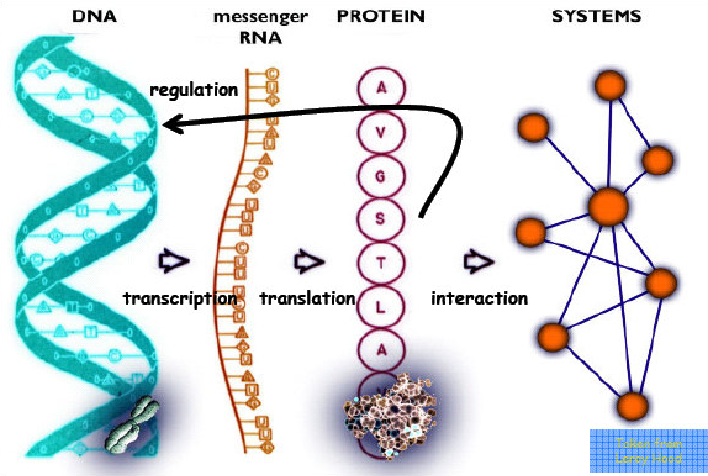
\includegraphics[height=3.5cm]{figs/dnascheme_white.png}
\end{center}

\pause
\begin{enumerate}[1)]
  \item Two main models
  \begin{itemize}
    \item Historical model: \tval{Biological Regulatory Network (René Thomas)}
    \item New developed model: \tval{Process Hitting}
  \end{itemize}

\medskip
  \item Allow efficient translation from Process Hitting to BRN
\end{enumerate}

\end{frame}


\section{Frameworks Definitions}
\subsection{The Process Hitting}
% Définition du Process Hitting + sortes coopératives

\begin{frame}[t]
  \frametitle{The Process Hitting modeling}
  \framesubtitle{\tcite{PMR12-MSCS}}

% 1 : Sortes
\only<1>{
\tikzstyle{process}=[circle,minimum size=15pt,font=\footnotesize,inner sep=1pt]
\tikzstyle{tick label}=[color=white, font=\footnotesize]
\tikzstyle{tick}=[transparent]
\tikzstyle{hit}=[transparent]
\tikzstyle{selfhit}=[transparent, min distance=30pt,curve to]
\tikzstyle{bounce}=[transparent]
\tikzstyle{hlhit}=[transparent]
\begin{center}\scalebox{\scaleex}{
\begin{tikzpicture}
\exphdef
\end{tikzpicture}
}\end{center}
}

% 2 : Processus
\only<2>{
\tikzstyle{process}=[circle,draw,minimum size=15pt,font=\footnotesize,inner sep=1pt]
\tikzstyle{tick label}=[font=\footnotesize]
\tikzstyle{tick}=[densely dotted]
\tikzstyle{hit}=[transparent]
\tikzstyle{selfhit}=[transparent, min distance=30pt,curve to]
\tikzstyle{bounce}=[transparent]
\tikzstyle{hlhit}=[transparent]
\begin{center}\scalebox{\scaleex}{
\begin{tikzpicture}
\exphdef
\end{tikzpicture}
}\end{center}
}

% 3 : États
\only<3>{
\tikzstyle{hit}=[transparent]
\tikzstyle{selfhit}=[transparent, min distance=30pt,curve to]
\tikzstyle{bounce}=[transparent]
\tikzstyle{hlhit}=[transparent]
\begin{center}\scalebox{\scaleex}{
\begin{tikzpicture}
\exphdef

\TState{3}{a_0,b_1,z_0}
\end{tikzpicture}
}\end{center}
}

% 4 : Actions
\only<4->{
\tikzstyle{tick}=[densely dotted]
\tikzstyle{hit}=[->,>=angle 45]
\tikzstyle{selfhit}=[min distance=30pt,curve to]
\tikzstyle{bounce}=[densely dotted,>=stealth',->]
\tikzstyle{hlhit}=[very thick]
\begin{center}\scalebox{\scaleex}{
\begin{tikzpicture}
\exphdef
\TState{4}{a_0,b_1,z_0}
\TState{5}{a_0,b_1,z_1}
\TState{6}{a_1,b_1,z_1}
\TState{7}{a_1,b_1,z_2}
\end{tikzpicture}
}\end{center}
}

\medskip
\begin{liste}
  \item \tval{Sorts}: components \qex{$a$, $b$, $z$}
\pause[2]
  \item \tval{Processes}: local states / levels of expression \qex{$z_0$, $z_1$, $z_2$}
\pause[3]
  \item \tval{States}: sets of active processes%
  \only<3-4>{\qex{$\PHetat{a_0, b_1, z_0}$}}%
  \only<5>{\qex{$\PHetat{a_0, b_1, z_1}$}}%
  \only<6>{\qex{$\PHetat{a_1, b_1, z_1}$}}%
  \only<7>{\qex{$\PHetat{a_1, b_1, z_2}$}}%
\pause[4]
  \item \tval{Actions}: dynamics \qex{\only<4>{\underline}{$\PHfrappe{b_1}{z_0}{z_1}$}, \only<4-5>{\underline}{$\PHfrappe{a_0}{a_0}{a_1}$}, \only<6>{\underline}{$\PHfrappe{a_1}{z_1}{z_2}$}}
\end{liste}
\end{frame}



\begin{frame}
  \frametitle{Adding cooperations}
  \framesubtitle{\tcite{PMR12-MSCS}}

\begin{center}\scalebox{\scaleex}{
\begin{tikzpicture}
\exphcoop
\end{tikzpicture}
}\end{center}

\medskip
\only<-14>{
\begin{liste}
  \item How to introduce some \tval{cooperation} between sorts? \qex{$\PHfrappe{a_1 \wedge b_0}{z_1}{z_2}$}
\pause[4]
  \item Solution: a \tval{cooperative sort} \qex{$ab$} \only<12->{\quad to express \qex{$a_1 \wedge b_0$}}
\pause[8]
  \item Constraint: each configuration is represented by one process \qex{$\PHetat{a_1,b_0} \pause[11]\Rightarrow ab_{10}$}
\pause[14]
  \item Advantage: regular sort; drawbacks: complexity, temporal shift
\end{liste}}
\end{frame}



\begin{frame}
  \frametitle{Static analysis: successive reachability}
  \framesubtitle{\tcite{PMR12-MSCS}}

Successive reachability of processes:

\begin{columns}
\begin{column}{0.55\textwidth}

\begin{center}
\scalebox{0.75}{
\begin{tikzpicture}
%\path[use as bounding box] (-1,-3) rectangle (7,2);
\exatt

\TState{2-4}{a_0,b_0,b_2,c_0,d_0}

\TState{5}{a_0,b_0,c_0,d_0}
\TState{6}{a_0,b_0,c_1,d_0}
\TState{7}{a_0,b_1,c_1,d_0}
\TState{8}{a_0,b_1,c_1,d_1}
\TState{9}{a_0,b_1,c_1,d_2}

\node<3>[process,very thick] (d_1) at (d_1.center) {1?};
\node<3>[process,very thick] (b_1) at (b_1.center) {2?};
\node<3>[process,very thick] (d_2) at (d_2.center) {3?};

\node<4-8>[process,very thick] (d_2) at (d_2.center) {1?};
\node<9>[process,very thick] (d_2) at (d_2.center) {};

\only<5>{\THit{a_0}{hlhit}{c_0}{.north}{c_1}}
\path<5>[bounce,bend left,hlhit] \TBounce{c_0}{}{c_1}{.west};
\only<6>{\THit{c_1}{bend left=20pt,hlhit}{b_0}{.west}{b_1}}
\path<6>[bounce,bend left,hlhit] \TBounce{b_0}{}{b_1}{.south};
\only<7>{\THit{b_0}{hlhit}{d_0}{.west}{d_1}}
\path<7>[bounce,bend left,hlhit] \TBounce{d_0}{}{d_1}{.south};
\only<8>{\THit{b_1}{hlhit}{d_1}{.west}{d_2}}
\path<8>[bounce,bend left,hlhit] \TBounce{d_1}{}{d_2}{.south};
\end{tikzpicture}
}
\end{center}

\end{column}
\begin{column}{0.45\textwidth}

\pause
~\\~\\~\\~\\
\begin{itemize}
  \item Initial context
    \\ \rex{\PHetat{a_1, \{b_0, b_1\}, c_0, z_0}} \pause
  \item Objectives
    \\ \rex{$[\ \Rsh d_1 \PHconcat\ \Rsh b_1 \PHconcat\ \Rsh d_2\ ]$} \pause
    \\\smallskip \rex{$[\ \Rsh d_2\ ]$} \pause
\end{itemize}

\end{column}
\end{columns}

\medskip
\begin{center}
\f Concretization of the objective = scenario

\ex{
\only<5>{\underline{$\PHfrappe{a_0}{c_0}{c_1}$}}\only<-4,6->{$\PHfrappe{a_0}{c_0}{c_1}$}~\PHconcat~
\only<6>{\underline{$\PHfrappe{b_0}{d_0}{d_1}$}}\only<-5,7->{$\PHfrappe{b_0}{d_0}{d_1}$}~\PHconcat~
\only<7>{\underline{$\PHfrappe{c_1}{b_0}{b_1}$}}\only<-6,8->{$\PHfrappe{c_1}{b_0}{b_1}$}~\PHconcat~
\only<8>{\underline{$\PHfrappe{b_1}{d_1}{d_2}$}}\only<-7,9->{$\PHfrappe{b_1}{d_1}{d_2}$}}
\end{center}

\end{frame}



\begin{frame}
  \frametitle{Over- and Under-approximations}
  \framesubtitle{\tcite{PMR12-MSCS}}

Static analysis by abstractions:
\begin{fleches}
  \item Directly checking an objective sequence $R$ is hard
  \item Rather check the approximations $P$ and $Q$, where \tval{$P \Rightarrow R \Rightarrow Q$}:
\end{fleches}

\begin{center}
\scalebox{0.6}{
\figsa
}
\end{center}

\only<-7>{~}
\only<8->{
Linear w.r.t.~the number of sorts and \\exponential w.r.t.~the number of processes in each sort
\begin{fleches}
  \item Efficient for big models with few levels of expression
\end{fleches}
}
\end{frame}



\begin{frame}[c]
  \frametitle{The Process Hitting modeling}

\begin{itemize}
  \item \tval{Dynamic} modeling with an \tval{atomistic} point of view
  \begin{fleches}
    \item Independent actions
    \item Cooperation modeled with cooperative sorts
  \end{fleches}

  \smallskip
  \item Efficient \tval{static analysis}
  \begin{fleches}
    \item Reachability of a process can be computed in \tval{linear time}\\
          \quad in the number of sorts
  \end{fleches}

  \smallskip
  \item Useful for the study of \tval{large biological models}
  \begin{fleches}
    \item Up to hundreds of sorts
  \end{fleches}

  \smallskip
  \item (Future) extensions
  \begin{fleches}
    \item Actions with stochasticity
    \item Actions with priorities
    \item Continuous time with clocks?
  \end{fleches}
\end{itemize}

\end{frame}


\subsection{Thomas' Modeling}
% Définition du modèle de Thomas

\colorlet{light}{colorgray}

\begin{frame}
  \frametitle{Biological Regulatory Network (Thomas' modeling)}
  \framesubtitle{\tcite{RCB08}}

\begin{tabular}{cccc}

\begin{tikzpicture}[grn]
\path[use as bounding box] (-0.7,-0.3) rectangle (2.5,2);
% Nœuds noirs
\only<1,3->{
  \node[inner sep=0] (z) at (2,0.75) {z};
  \node[inner sep=0] (a) at (0,1.5) {a};
  \node[inner sep=0] (b) at (0,0) {b};
  \path
    node[elabel, below=-1em of a] {$0..1$}
    node[elabel, below=-1em of b] {$0..1$}
    node[elabel, below=-1em of z] {$0..2$};}
% Nœuds grisés
\only<2>{
  \node[inner sep=0,light] (z) at (2,0.75) {z};
  \node[inner sep=0,light] (a) at (0,1.5) {a};
  \node[inner sep=0,light] (b) at (0,0) {b};
  \path
    node[elabel, below=-1em of a,light] {$0..1$}
    node[elabel, below=-1em of b,light] {$0..1$}
    node[elabel, below=-1em of z,light] {$0..2$};}

% Arcs colorés
\only<1,4->{\path
  (a) edge[inh,loop left=10] node[elabel, left] {$1-$} (a)
  (a) edge[act] node[elabel, above=-2pt] {$1+$} (z)
  (b) edge[inh] node[elabel, below=-2pt] {$1-$} (z);}
% Arcs grisés
\only<2-3>{\path
  (a) edge[inhgray,loop left=10] node[elabel, left,light] {$1-$} (a)
  (a) edge[actgray] node[elabel, above=-2pt,light] {$1+$} (z)
  (b) edge[inhgray] node[elabel, below=-2pt,light] {$1-$} (z);}
\end{tikzpicture}
&%
\only<2-4>{\color{light}}%
\begin{tabular}[b]{c|c|c}
  \multicolumn{2}{c|}{$\omega$} & \multirow{2}{*}{$k_{z, \omega}$} \\
\cline{1-2}
  $a$ & $b$ & \\
\hline
  $-$ & $+$ & $1$ \\
  $-$ & $-$ & $0$ \\
  \only<6>{\color{red}}$+$ & \only<6>{\color{red}}$+$ & \only<6>{\color{red}}$2$ \\
  $+$ & $-$ & $1$
\end{tabular}
%\begin{tabular}[b]{c|c}
%  $\omega$ & $k_{z, \omega}$ \\
%\hline
%  $\emptyset$ & $1$ \\
%  $\{b\}$ & $0$ \\
%  \only<7-8>{\color{red}}$\{a\}$ & \only<7-8>{\color{red}}$2$ \\
%  $\{a;b\}$ & $1$
%\end{tabular}
~~~~&
\only<2-4>{\color{light}}%
\begin{tabular}[b]{c|c}
  $\omega$ & \multirow{2}{*}{$k_{a, \omega}$} \\
\cline{1-1}
  $a$ & \\
\hline
  $+$ & $1$ \\
  $-$ & $0$
\end{tabular}
%\begin{tabular}[b]{c|c}
%  $\omega$ & $k_{a, \omega}$ \\
%\hline
%  $\emptyset$ & $1$ \\
%  $\{a\}$ & $0$
%\end{tabular}
&
\only<2-4>{\color{light}}%
\begin{tabular}[b]{cc}
  & $k_{b, \omega}$ \\
\cline{2-2}
  & $1$
\end{tabular}
%\begin{tabular}[b]{c|c}
%  $\omega$ & $k_{b, \omega}$ \\
%\hline
%  $\emptyset$ & $1$
%\end{tabular}
\\
\only<2-4>{$\underbrace{\text{\hspace{3cm}}}_{\text{Interaction Graph}}$}%
&
\multicolumn{3}{r}{\only<5->{$\underbrace{\text{\hspace{6.5cm}}}_\text{Parametrization}$}}
\end{tabular}

\bigskip
% Historical model...
\only<1>{

\bigskip
Proposed by René Thomas in 1973, several extensions since then
\medskip
\begin{liste}
  \item \tval{Historical bio-informatics model} for studying genes interactions
  \item Widely used and well-adapted to represent dynamic gene systems
\end{liste}
}

% Interaction Graph
\only<2-4>{
\tval{Interaction Graph}: structure of the system (genes \& interactions)

\pause[3]
\medskip
\begin{liste}
  \item \tval{Nodes}: genes
  \begin{fleches}
    \item Name \qex{$a$, $b$, $z$}
    \item Possible values (levels of expression) \qex{$0..1$, $0..2$}
  \end{fleches}
\pause[4]
  \item \tval{Edges}: interactions
  \begin{fleches}
    \item Threshold \qex{$1$}
    \item Type (activation or inhibition) \qex{$+$ / $-$}
  \end{fleches}
\end{liste}
}

% Parametrization
\only<5->{
\medskip
\tval{Parametrization}: strength of the influences (cooperations)

\medskip
\begin{liste}
  \item Maps of tendencies for each gene
  \begin{fleches}
    \item To any \tval{influences of predecessors} \qex{$\omega$}
    \item Corresponds a \tval{parameter} \qex{$k_{x,\omega}$}
  \end{fleches}
\pause[6]
\medskip
  \item \ex{“$k_{z, \{a^+, b^+\}} = 2$”} \quad means: \qex{“$z$ tends to $2$ when $a \geq 1$ and $b < 1$”}
%  \item \ex{“$k_{z, \{a\}} = [2;2]$”} \quad means: \qex{“$z$ tends to \only<7>{$[2;2]$}\only<8->{$2$} when $a \only<7>{\geq}\only<8->{=} 1$ and $b \only<7>{< 1}\only<8->{= 0}$”}
\end{liste}
%\pause[10]
}\end{frame}



\begin{frame}
  \frametitle{Biological Regulatory Network (Thomas' modeling)}
  \framesubtitle{\tcite{RCB08}}

\begin{tabular}{cccc}

\begin{tikzpicture}[grn]
\path[use as bounding box] (-0.7,-0.3) rectangle (2.5,2);
\node[inner sep=0] (z) at (2,0.75) {z};
\node[inner sep=0] (a) at (0,1.5) {a};
\node[inner sep=0] (b) at (0,0) {b};
\path
  node[elabel, below=-1em of a] {$0..1$}
  node[elabel, below=-1em of b] {$0..1$}
  node[elabel, below=-1em of z] {$0..2$};
\path
  (a) edge[inh,loop left=10] node[elabel, left] {$1-$} (a)
  (a) edge[act] node[elabel, above=-2pt] {$1+$} (z)
  (b) edge[inh] node[elabel, below=-2pt] {$1-$} (z);
\end{tikzpicture}
&
\begin{tabular}[b]{c|c|c}
  \multicolumn{2}{c|}{$\omega$} & \multirow{2}{*}{$k_{z, \omega}$} \\
\cline{1-2}
  $a$ & $b$ & \\
\hline
  $-$ & $+$ & $1$ \\
  $-$ & $-$ & $0$ \\
  $+$ & $+$ & $2$ \\
  $+$ & $-$ & $1$
\end{tabular}
~~~~&
\begin{tabular}[b]{c|c}
  $\omega$ & \multirow{2}{*}{$k_{a, \omega}$} \\
\cline{1-1}
  $a$ & \\
\hline
  $+$ & $1$ \\
  $-$ & $0$
\end{tabular}
&
\begin{tabular}[b]{cc}
   & $k_{b, \omega}$ \\
\cline{2-2}
   & $1$
\end{tabular}
\\
\multicolumn{4}{r}{$\underbrace{\text{\hspace{10.1cm}}}_{\text{Biological Regulatory Network}}$}
\end{tabular}

\bigskip

\begin{itemize}
  \item[\f] All needed information to run the model or study its dynamics:
  \begin{itemize}\normalsize
    \item Build the State Graph
    \item Find reachability properties, fixed points, attractors
    \item Other properties...
  \end{itemize}
\end{itemize}

\begin{itemize}
  \item[\f] \tval{Strengths}: well adapted for the study of biological systems
  \item[\f] \tval{Drawbacks}: inherent complexity; needs the full\\
    \quad \quad specification of cooperations
\end{itemize}
\end{frame}


%%%\subsection{Answer Set Programming}
%%%% Pistes d'implémentation

\begin{frame}[c]
  \frametitle{ASP Implementation}

\tval{ASP}: Declarative programming

\quad Rule: \ex{$head \leftarrow \only<1>{body}\only<2->{A_1, ..., A_n, \neg A_{n+1}, ..., \neg A_m}.$}

\quad Fact: \ex{$head.$}

\quad Constraint: \ex{$\leftarrow body.$}

\quad Aggregate: \ex{$lower~\{~atoms~\}~upper \leftarrow body.$}

\pause[3]
\bigskip
Representation of PH / BRNs:

\quad Gene: \ex{$component(a, n).$}

\quad Action: \ex{$action(a, i, b, j, k).$}

\quad Cooperation: \ex{$cooperation(c, a, i, j).$}

\quad Useful rules: \ex{$component\_levels(X, 0..M) \leftarrow component(X, M).$}
\end{frame}


\section{Translating a Process Hitting into a BRN}
% Introduction à la traduction

\begin{frame}[c]
  \frametitle{Inferring a BRN with Thomas' parameters}
  \framesubtitle{~}

\begin{center}
\scalebox{\scaleinf}{
\begin{tikzpicture}
\path[use as bounding box] (-0.5,-0.8) rectangle (6.5,4);
\exphinfblack
\end{tikzpicture}
}
\end{center}

\begin{center}
\begin{tikzpicture}
\path[use as bounding box] (1,1) rectangle (4,1.5);
\only<2->{
  \path[draw] (1, 1.8) edge[->,draw,very thick] node[left=3pt,circle,draw=black,outer sep=2pt,minimum size=15pt,text=black] {1} (0, 0);}

\only<3->{
\node[circle,draw=black,inner sep=0,minimum size=5pt,fill=black] (s2) at (2,0.7) {};
\node[left=4pt of s2,circle,draw=black,outer sep=2pt,minimum size=15pt,text=black,very thick] (e2) at (2,0.8) {2};
\path[draw] (2.25, 1.8) edge[draw,very thick] (s2);
\path[draw] (1, -0.25) edge[draw,very thick] (s2);
\path[draw] (s2) edge[->,draw,very thick] (3.75, 0);}
\end{tikzpicture}
\end{center}

\begin{columns}
\begin{column}{0.6\textwidth}

\begin{center}
\begin{tikzpicture}[grn]
\path[use as bounding box] (0.5,-0.5) rectangle (2,1.5);
% Gènes noirs
\only<2->{
  \node[inner sep=0] (a) at (0,1.5) {a};
  \node[inner sep=0] (b) at (0,0) {b};
  \node[inner sep=0] (z) at (2,0.75) {z};}
% Gènes gris
\only<1>{
  \node[inner sep=0,colorgray] (a) at (0,1.5) {a};
  \node[inner sep=0,colorgray] (b) at (0,0) {b};
  \node[inner sep=0,colorgray] (z) at (2,0.75) {z};}

% Arcs colorés
\only<2->{
  \path (a) edge[act] node[elabel,above=-2pt] {$1+$} (z);
  \path (b) edge[inh] node[elabel,below=-2pt] {$1-$} (z);}
% Arcs grisés
\only<1>{
  \path (a) edge[actgray] node[elabel,above=-2pt,colorgray] {$1+$} (z);
  \path (b) edge[inhgray] node[elabel,below=-2pt,colorgray] {$1-$} (z);}
\end{tikzpicture}
\end{center}

\end{column}
\begin{column}{0.4\textwidth}

\only<1-2>{\color{colorgray}}
\begin{tabular}{c|c}
  $\omega$ & $k_{z, \omega}$ \\
\hline
  $\emptyset$ & $1$ \\
  $\{b\}$ & $0$ \\
  $\{a\}$ & $2$ \\
  $\{a;b\}$ & $1$
\end{tabular}

\end{column}
\end{columns}


\end{frame}

\subsection{Interaction Graph Inference}
% Inférence du Graphe des Interactions



\begin{frame}
  \frametitle{Inferring the Interaction Graph}
  \framesubtitle{\tcite{CMSB12}}

\begin{columns}
\begin{column}{0.65\textwidth}

\begin{center}\scalebox{\scaleinf}{
\begin{tikzpicture}
\path[use as bounding box] (-0.5,-0.8) rectangle (6.5,2.8);
\exphinf

% Processus marqués
\only<4-9>{\node[current process,fill=colorb] (hb_0) at (b_0.center) {};}
\only<5-9>{
  \node[current process,fill=colora1] (ha_1) at (a_1.center) {};
  \node[current process,fill=colora1] (hab_2) at (ab_2.center) {};}
\only<6-9>{
  \node[current process,fill=colora1] (hz_2) at (z_2.center) {};}
\only<7-9>{
  \node[current process,fill=colora0] (ha_0) at (a_0.center) {};
  \node[current process,fill=colora0] (hab_0) at (ab_0.center) {};}
\only<8-9>{
  \node[current process,fill=colora0] (hz_0) at (z_0.center) {};}

\only<10->{\node[current process,fill=colorb] (hb_1) at (b_1.center) {};}
\only<10->{
  \node[current process,fill=colora1] (ha_1) at (a_1.center) {};
  \node[current process,fill=colora1] (hab_3) at (ab_3.center) {};
  \node[current process,fill=colora0] (ha_0) at (a_0.center) {};
  \node[current process,fill=colora0] (hab_1) at (ab_1.center) {};}
\only<11->{
  \node[current process,fill=colora1] (hz_1) at (z_1.center) {};
  \node[current process,fill=colora0,inner sep=0,minimum size=7pt,draw=none] (hz_1bis) at (z_1.center) {};}

% Actions mises en valeur
\only<5-6>{
  \THit{ab_2}{}{z_1}{.north west}{z_2}
  \THit{ab_2}{}{z_0}{.west}{z_1}
  \path[bounce,bend left] \TBounce{z_1}{}{z_2}{.south} \TBounce{z_0}{}{z_1}{.south} ;}
\only<7-8>{
  \THit{ab_0}{}{z_2}{.west}{z_1}
  \THit{ab_0}{}{z_1}{.south west}{z_0}
  \path[bounce,bend right] \TBounce{z_2}{}{z_1}{.north} \TBounce{z_1}{}{z_0}{.north} ;}
\only<10->{
  \THit{ab_3}{}{z_2}{.west}{z_1}
  \THit{ab_3}{}{z_0}{.west}{z_1}
  \THit{ab_1}{}{z_2}{.west}{z_1}
  \THit{ab_1}{}{z_0}{.west}{z_1}
  \path[bounce,bend left] \TBounce{z_2}{bend right}{z_1}{.north} \TBounce{z_0}{}{z_1}{.south} ;}

\end{tikzpicture}
}\end{center}

\end{column}
\begin{column}{0.45\textwidth}

\begin{center}
\begin{tikzpicture}[grn]
\path[use as bounding box] (1,-0.5) rectangle (2.5,1.5);
% Gènes noirs
\only<1->{\node[inner sep=0] (a) at (0,1.5) {a};}
\only<1-3>{\node[inner sep=0] (b) at (0,0) {b};}
\only<1->{\node[inner sep=0] (z) at (2,0.75) {z};}
%\only<1-2>{\path node[elabel, below=-1em of a] {$0..1$}; \path node[elabel, below=-1em of b] {$0..1$}; \path node[elabel, below=-1em of z] {$0..2$};}
% Gènes gris
%\only<3>{\node[colorgray,inner sep=0] (a) at (0,1.5) {a};}
\only<4->{\node[colorgray,inner sep=0] (b) at (0,0) {b};}

%\newcolumntype{M}[1]{>{\raggedright}m{#1}}

% Arc noir
\only<2-12>{\path (a) edge[inf] node[elabel,above right=-2.4em,font=\scriptsize] {\begin{tabular*}{3cm}{c}%
$\color{white}\left\{\color{black}\text{\begin{tabular*}{1.7cm}{l}%
  $\only<10->{\{b = 1\} \only<15>{\phantom{\Rightarrow \sim}}\only<12->{\Rightarrow {\color{exanswer}\sim}}}$\tabularnewline%
  $\only<4->{\{b = 0\} \only<9->{\Rightarrow {\color{exanswer}1+}}}$%
\end{tabular*}}\only<-16>{\right.}\only<17->{\right\}\textcolor{exanswer}{1+}}$%
\end{tabular*}} (z) ;}
\only<2-3>{\path (b) edge[inf] node[elabel, below=-2pt] {$\only<99->{-\!\only<1->{1}}$} (z) ;}
% Arc coloré
\only<13->{\path (a) edge[act,very thick,notsodarkgreen] node[elabel,above right=-2.4em,font=\scriptsize] {\begin{tabular*}{3cm}{c}%
$\color{white}\left\{\color{black}\text{\begin{tabular*}{1.7cm}{l}%
  $\only<10->{\{b = 1\} \only<11>{\phantom{\Rightarrow \sim}}\only<12->{\Rightarrow {\color{exanswer}\sim}}}$\tabularnewline%
  $\only<4->{\{b = 0\} \only<9->{\Rightarrow {\color{exanswer}1+}}}$%
\end{tabular*}}\only<13->{\right\}\textcolor{exanswer}{1+}}$%
\end{tabular*}} (z) ;}
% Arcs gris
%\only<3>{\path (a) edge[inf,draw=colorgray,fill=colorgray] node[colorgray,elabel, above=-2pt] {$\only<1>{+\!\only<2->{1}}$} (z) ;}
\only<4->{\path (b) edge[inf,draw=colorgray,fill=colorgray] node[colorgray,elabel, below=-2pt] {$\only<1>{-\!\only<1->{1}}$} (z) ;}
\end{tikzpicture}
\end{center}

\end{column}
\end{columns}

\bigskip

% Méthode
\pause[3]
\f \tval{Exhaustive search in all possible configurations}

\pause
\begin{enumerate}[1.]
  \item Pick one regulator [\ex{$a$}], and choose an active process for all the others [\ex{$b_0$}].
\pause
  \item Change the active process of this regulator [\ex{$a_0$}, \ex{$a_1$}] and watch the \tval{focal processes}.
\pause[9]
  \item Conclude locally: ($\textcolor{colora0font}{a_0} \Rsh \textcolor{colora1font}{a_1} \Rightarrow \textcolor{colora0font}{z_0} \Rsh \textcolor{colora1font}{z_2}$)
      $\Rightarrow \text{activation (}\textcolor{exanswer}{+}\text{) \& threshold = \ex{$1$}}$.
\pause
  \item Iterate \only<13->{and conclude globally.}
\end{enumerate}

\pause[14]
\smallskip
Problematic cases:\\
\smallskip
$\left.\text{\begin{tabular}{l}
  \f No focal processes (cycle)\\
  \f Opposite influences (\ex{$+$} \& \ex{$-$})
 \end{tabular}}\right\} \Rightarrow \text{ Unsigned edge}$
\end{frame}

\subsection{Parametrization Inference}
% Inférence de la Paramétrisation

\begin{frame}
  \frametitle{Inferring Parameters}
  \framesubtitle{\tcite{PMR10-TCSB}}

\begin{columns}
\begin{column}{0.5\textwidth}

\only<1-5>{
\begin{center}
\scalebox{\scaleinf}{
\begin{tikzpicture}
\path[use as bounding box] (-0.5,-0.8) rectangle (6.5,2.8);
\exphinf

% Processus mis en valeur
\only<2->{
  \node[current process,fill=colorb] (hb_1) at (b_1.center) {};
  \node[current process,fill=colorb] (ha_1) at (a_1.center) {};}
\only<2->{
  \node[current process,fill=colorb] (hab_3) at (ab_3.center) {};}
\only<3->{
  \node[current process,fill=colorb] (hz_1) at (z_1.center) {};}

% Actions mises en valeur
\only<3->{
  \THit{ab_3}{}{z_2}{.west}{z_1}
  \THit{ab_3}{}{z_0}{.west}{z_1}
  \path[bounce,bend left] \TBounce{z_2}{bend right}{z_1}{.north} \TBounce{z_0}{}{z_1}{.south};}
\end{tikzpicture}
}
\end{center}
}

\only<6->{
\begin{center}
\scalebox{\scaleinf}{
\begin{tikzpicture}
\path[use as bounding box] (-0.5,-0.8) rectangle (6.5,2.8);
\exphinfprojssc

% Processus mis en valeur
\only<2->{
  \node[current process,fill=colorb] (hb_1) at (b_1.center) {};
  \node[current process,fill=colorb] (ha_1) at (a_1.center) {};}

% Actions mises en valeur
\only<2->{
  \THit{a_1}{}{z_0}{.west}{z_1}
  \THit{a_1}{}{z_1}{.north west}{z_2}
  \THit{b_1}{}{z_1}{.south west}{z_0}
  \THit{b_1}{}{z_2}{.west}{z_1}
  \path[bounce,bend left] \TBounce{z_0}{}{z_1}{.south} \TBounce{z_1}{}{z_2}{.south}
    \TBounce{z_1}{bend right}{z_0}{.north} \TBounce{z_2}{bend right}{z_1}{.north} ;}

\end{tikzpicture}
}
\end{center}
}

\end{column}
\begin{column}{0.2\textwidth}

\begin{center}
\begin{tikzpicture}[grn]
\path[use as bounding box] (0.5,-0.5) rectangle (2,1.5);
% Gènes noirs
  \node[inner sep=0] (a) at (0,1.5) {a};
  \node[inner sep=0] (b) at (0,0) {b};
  \node[inner sep=0] (z) at (2,0.75) {z};
% Arcs colorés
  \path (a) edge[act] node[elabel,above=-2pt] {$1+$} (z) ;
  \path (b) edge[inh] node[elabel,below=-2pt] {$1-$} (z) ;
\end{tikzpicture}
\end{center}

\end{column}
\begin{column}{0.25\textwidth}

\only<1-5>{
\begin{tabular}{c|c|c}
%  $\omega$ & $k_{z, \omega}$ \\
%\hline
  \multicolumn{2}{c|}{$\omega$} & \multirow{2}{*}{$k_{z, \omega}$} \\
\cline{1-2}
  $a$ & $b$ & \\
\hline
  \only<2->{\color{colorgray}}$-$ & \only<2->{\color{colorgray}}$+$ & \\
  \only<2->{\color{colorgray}}$-$ & \only<2->{\color{colorgray}}$-$ & \\
  \only<2->{\color{colorgray}}$+$ & \only<2->{\color{colorgray}}$+$ & \\
  \only<1>{$+$}\only<2->{\redex{$+$}} & \only<1>{$-$}\only<2->{\redex{$-$}} & \uncover<4->{\redex{$1$}}
\end{tabular}
}

\only<6->{
\begin{tabular}{c|c|c}
%  $\omega$ & $k_{z, \omega}$ \\
%\hline
  \multicolumn{2}{c|}{$\omega$} & \multirow{2}{*}{$k_{z, \omega}$} \\
\cline{1-2}
  $a$ & $b$ & \\
\hline
  $-$ & $+$ & \redex{\textit{?}} \\ %\textcolor{lightgray}{\textit{?}} \\
  $-$ & $-$ & $0$ \\
  $+$ & $+$ & $2$ \\
  $+$ & $-$ & \redex{\textit{?}} %\textcolor{lightgray}{\textit{?}}
\end{tabular}
}

\end{column}
\end{columns}

\bigskip
\pause[2]
\begin{enumerate}[1.]
  \item For each configuration of resources \quad [\ex{$\omega = \{a^+, b^-\}$}]\\
\pause
        find the \tval{focal processes}.\pause[4] If possible, conclude. \quad [$\ex{k_{z,\{a^+, b^-\}} = 1}$]
\pause[5]
 \item[] Inconclusive cases:
  \begin{itemize}
    \item[--] Behavior cannot be represented as a BRN
    \item[--] Lack of cooperation (no focal processes)
  \end{itemize}
\medskip
\pause
  \item If some parameters could not be inferred, enumerate all admissible parametrizations, regarding:
  \begin{itemize}
    \item[--] Biological constraints
    \item[--] The dynamics of the Process Hitting
  \end{itemize}
  \hfill[\ex{$k_{z, \{a^+, b^-\}} \in \{0 ; 1 ; 2\}$}; \ex{$k_{z, \{a^-, b^+\}} \in \{0 ; 1 ; 2\}$}]
\end{enumerate}
\end{frame}


\begin{comment}
\begin{frame}[c]
  \frametitle{Parametrization Inference}
  \framesubtitle{Results}

Two steps:
\begin{itemize}
  \item Parameters inference (partial)
  \item Admissible Parametrizations enumeration (total)
\end{itemize}


\medskip

\pause

\tval{Results}:
\begin{itemize}
  \item Very fast execution for parameters inference
  \begin{itemize}
    \item[] \tval{$<$ 1s} for the 20 \& 40 genes models \quad\tval{\ex{[EGFR20 \& TCRSIG40]}}
%\f all 191 \& 141 parameters
    \item[] \tval{$\simeq$ 1min 30s} for the 104 genes models \quad\tval{\ex{[EGFR104]}}
%    \item[] \quad\quad (solving only) \f found $2.10^6 / 4.10^6$ parameters
  \end{itemize}
  \item Admissible Parametrizations enumeration
  \begin{itemize}
    \item[] After one cooperation removal:
    \item[] \quad $\simeq$ \tval{4s} to find 42 admissible Parametrizations \quad\tval{\ex{[TCRSIG40]}}
    \item[] \quad $\simeq$ \tval{20s} to find 129 admissible Parametrizations \quad\tval{\ex{[EGFR20]}}
  \end{itemize}
\end{itemize}

\medskip
ASP is convenient to handle enumeration (\tval{cardinalities})

and filter only admissible answers (\tval{constraints})

\end{frame}
\end{comment}


\section{Summary \& Conclusion}
% Performances et conclusion


\begin{frame}[c]
  \frametitle{Implementation}

\small
\tval{Workflow}:
\begin{itemize}
  \item Read and translate the models with \tval{OCaml}\\
        \quad\f Uses the existing free library \tval{Pint}\\
        \quad\f Documentation + examples: \lien{http://processhitting.wordpress.com/}
  \item Express the problem in \tval{ASP} (logic programming)\\
        \quad\f Solve with \tval{Clingo} (\tval{Gringo} + \tval{Clasp})
\end{itemize}

\pause
\bigskip
\begin{tabular}{c||r@{+}l|c|c||c|c||c|c|}
\multicolumn{5}{c||}{Model specifications} & \multicolumn{2}{c||}{IG inference} & \multicolumn{2}{c|}{Parameters inference}\\
\hline
\tval{Name} & S & CS & P & A & $\Delta t$ & Edges & $\Delta t$ & Parameters\\
\hline
  \tval{\ex{[EGFR20]}} & \tval{20} & 22 & 152 & 399 & \tval{1s} & 50 & \tval{1s} & 191\\
\hline
  \tval{\ex{[TCRSIG40]}} & \tval{40} & 14 & 156 & 301 & \tval{1s} & 54 & \tval{1s} & 143\\
\hline
  \tval{\ex{[TCRSIG94]}} & \tval{94} & 39 & 448 & 1124 & \tval{13s} & 169 & $\infty$ & $2.10^9$\\
\hline
  \tval{\ex{[EGFR104]}} & \tval{104} & 89~ & 748 & 2356 & \tval{4min} & 241 & \tval{1min 30s} & $1.10^6 / 2.10^6$\\
\hline
\end{tabular}

S = Sorts \quad CS = Cooperative sorts \quad P = Processes \quad A = Actions

\bigskip
\quad\tval{\ex{[EGFR20]}}: Epidermal Growth Factor Receptor, by Özgür Sahin et al.\\
\quad\tval{\ex{[EGFR104]}}: Epidermal Growth Factor Receptor, by Regina Samaga et al.\\
\quad\tval{\ex{[TCRSIG40]}}: T-Cell Receptor Signaling, by Steffen Klamt et al.\\
\quad\tval{\ex{[TCRSIG94]}}: T-Cell Receptor Signaling, by Julio Saez-Rodriguez et al.

\end{frame}



\begin{frame}[c]
  \frametitle{Summary}

\begin{enumerate}[1.]
  \item Inference of the \tval{complete Interaction Graph}
  \item Inference of the \tval{possibly partial Parametrization}
  \item Enumerate all full \& \tval{admissible Parametrizations}
\end{enumerate}
\quad\quad\f Exhaustive approaches

\bigskip
\tval{Complexity}: linear in the number of genes, exponential in the number of regulators of one gene

\pause
\bigskip
\begin{flushright}
\Large
\textcolor{couleurtheme}{Conclusion}\hspace*{2.7em}
\end{flushright}

\medskip
Existing translation: René Thomas $\rightsquigarrow$ Process Hitting

\smallskip
New translation: Process Hitting $\rightsquigarrow$ René Thomas

\smallskip
\begin{fleches}
  \item New \tval{formal link} between the two models
  \item More \tval{visibility} to the Process Hitting
\end{fleches}
\end{frame}



\begin{frame}[c]
  \frametitle{A multi-team topic}

\tval{Inoue Laboratory} (NII, Sokendai): Constraint Programming, Systems Biology

\tval{MeForBio} (IRCCyN, ÉCN): Formal Methods for Bioinformatics

\tval{AMIB} (LIX, Polytechnique): Algorithms and Models for Integrative Biology

\bigskip\bigskip\footnotesize
\begin{tabular}{cc}
  $\left.\text{\begin{tabular}{c}
    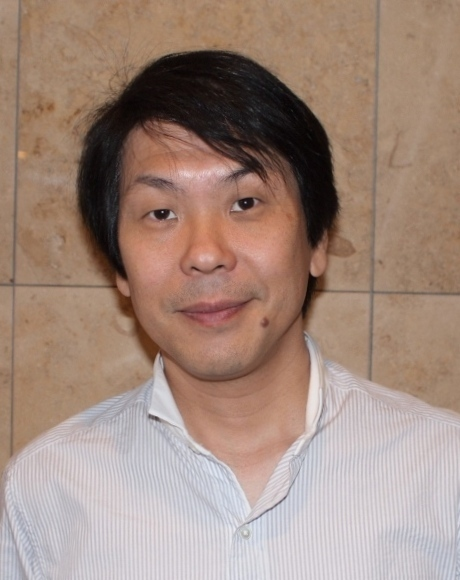
\includegraphics[height=1.5cm]{figs/Inoue-sensei.jpg} \\ \tval{Katsumi INOUE} \\ Professor \& team leader
  \end{tabular}}\right\}\text{\tval{Inoue Laboratory}}$
  &
  $\left.\text{\begin{tabular}{c}
    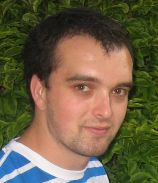
\includegraphics[height=1.5cm]{figs/Loic.jpg} \\ \tval{Loïc PAULEVÉ} \\ Post-doc
  \end{tabular}}\right\}\text{\tval{AMIB}}$
  \\ & \\ & \\
  \multicolumn{2}{l}{$\left.\text{\begin{tabular}{ccc}
      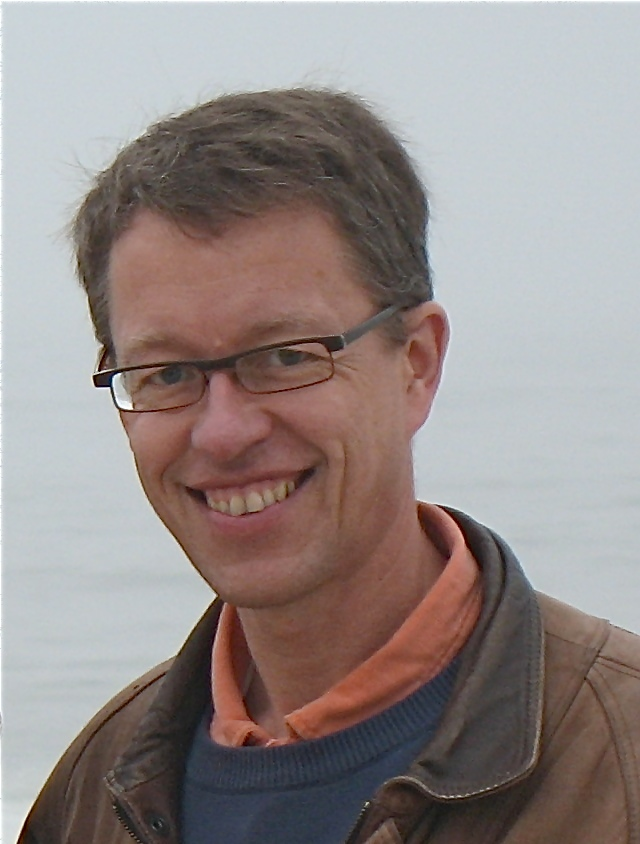
\includegraphics[height=1.5cm]{figs/Olivier.jpg}
    & 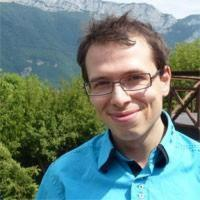
\includegraphics[height=1.5cm]{figs/Morgan.jpg}
    & 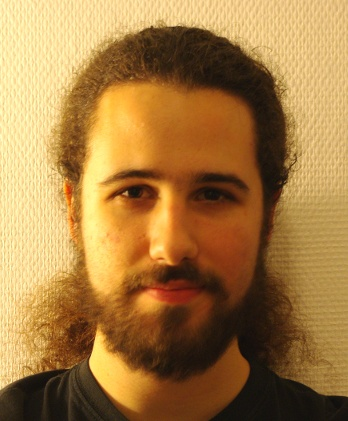
\includegraphics[height=1.5cm]{figs/Moi.jpg} \\
      \tval{Olivier ROUX} & \tval{Morgan MAGNIN} & \tval{Maxime FOLSCHETTE} \\
      Professor \& team leader & Associate professor & 2\textsuperscript{nd} year PhD student
  \end{tabular}}\right\}\text{\tval{MeForBio}}$}
\end{tabular}
\end{frame}

\appendix
\section[x]{Bibliography}
% Bibliographie

\begin{frame}[c]
  \frametitle{Bibliography}

\footnotesize
\setlength{\parindent}{-1em}
\setlength{\parskip}{0.5em}
~

\vfill

\tcite{PMR10-TCSB} Loïc Paulevé, Morgan Magnin, Olivier Roux. \ex{Refining dynamics of gene regulatory networks in a stochastic $\pi$-calculus framework}. In Corrado Priami, Ralph-Johan Back, Ion Petre, and Erik de Vink, editors: \textit{Transactions on Computational Systems Biology XIII}, volume 6575 of Lecture Notes in Computer Science, 171-191. Springer Berlin/Heidelberg, 2011.

\tcite{PMR12-MSCS} Loïc Paulevé, Morgan Magnin, Olivier Roux. \ex{Static analysis of biological regulatory networks dynamics using abstract interpretation}. \textit{Mathematical Structures in Computer Science}, 2012.

\tcite{RCB08} Adrien Richard, Jean-Paul Comet, Gilles Bernot. \ex{R. Thomas' logical method}, 2008. Invited at \textit{Tutorials on modelling methods and tools: Modelling a genetic switch and Metabolic Networks}, Spring School on Modelling Complex Biological Systems in the Context of Genomics.

\tcite{CMSB12} Maxime Folschette, Loïc Paulevé, Katsumi Inoue, Morgan Magnin, Olivier Roux. \ex{Concretizing the Process Hitting into Biological Regulatory Networks}. In David Gilbert and Monika Heiner, editors, \textit{Computational Methods in Systems Biology X}, Lecture Notes in Computer Science, pages 166–186. Springer Berlin
Heidelberg, 2012.

%\tcite{Paulevé11} Loïc Paulevé. PhD thesis: \ex{\textit{Modélisation, Simulation et Vérification des Grands Réseaux de Régulation Biologique}}, October 2011, Nantes, France

%\tcite{PMR10-TSE} Loïc Paulevé, Morgan Magnin, and Olivier Roux. \textit{Tuning Temporal Features within the Stochastic $\pi$-Calculus}. IEEE Transactions on Software Engineering, 37(6):858-871, 2011.

%\tcite{PR10-CRAS} Loïc Paulevé and Adrien Richard. \textit{Topological Fixed Points in Boolean Networks}. Comptes Rendus de l'Académie des Sciences - Series I - Mathematics, 348(15-16):825 - 828, 2010.

\vfill
\Large
\begin{flushright}
  \tval{Thank you}\hspace{1cm}~
\end{flushright}
\vfill

~

\end{frame}


\end{document}
